\documentclass[12pt]{article}
\renewcommand{\thesection}{\Roman{section}} 
\renewcommand{\thesubsection}{\thesection.\Roman{subsection}}
%\usepackage[tocindentauto]{tocstyle}
%\usetocstyle{KOMAlike} %the previous line resets it
%\usepackage{natbib}
\usepackage{biblatex}
\addbibresource[]{ref.bib}
\usepackage{url}
\usepackage[utf8]{inputenc}
\usepackage{amsmath}
\usepackage{graphicx}
\usepackage{graphviz}
\usepackage[T1]{fontenc}
\graphicspath{{images/}}
\usepackage{parskip}
\usepackage{fancyhdr}
\usepackage{hyperref}
\usepackage{parskip}
\usepackage{hologo}
\usepackage{listings}
\usepackage{titlesec, blindtext, color}
\usepackage{titling}
\usepackage{tcolorbox}
\usepackage[hmargin=1in,vmargin=1in]{geometry}
\usepackage{float}
\usepackage{tikz}
\usepackage{appendix}
\usepackage{listings} % For code importing
\usepackage{xcolor} % for setting colors
\usepackage{svg}
\usepackage{tocloft}
\renewcommand{\cftsecleader}{\cftdotfill{\cftdotsep}}

 %%%%%%%%%%%%%%%%%%%%%%%%%%%%%%%%%%%%%%%%%%%%%%%%%%%%%%%%%%%%%%%%%%%%%%%%%%%%%%%% 
%%% ~ Arduino Language - Arduino IDE Colors ~                                  %%%
%%%                                                                            %%%
%%% Kyle Rocha-Brownell | 10/2/2017 | No Licence                               %%%
%%% -------------------------------------------------------------------------- %%%
%%%                                                                            %%%
%%% Place this file in your working directory (next to the latex file you're   %%%
%%% working on).  To add it to your project, place:                            %%%
%%%     %%%%%%%%%%%%%%%%%%%%%%%%%%%%%%%%%%%%%%%%%%%%%%%%%%%%%%%%%%%%%%%%%%%%%%%%%%%%%%%% 
%%% ~ Arduino Language - Arduino IDE Colors ~                                  %%%
%%%                                                                            %%%
%%% Kyle Rocha-Brownell | 10/2/2017 | No Licence                               %%%
%%% -------------------------------------------------------------------------- %%%
%%%                                                                            %%%
%%% Place this file in your working directory (next to the latex file you're   %%%
%%% working on).  To add it to your project, place:                            %%%
%%%     %%%%%%%%%%%%%%%%%%%%%%%%%%%%%%%%%%%%%%%%%%%%%%%%%%%%%%%%%%%%%%%%%%%%%%%%%%%%%%%% 
%%% ~ Arduino Language - Arduino IDE Colors ~                                  %%%
%%%                                                                            %%%
%%% Kyle Rocha-Brownell | 10/2/2017 | No Licence                               %%%
%%% -------------------------------------------------------------------------- %%%
%%%                                                                            %%%
%%% Place this file in your working directory (next to the latex file you're   %%%
%%% working on).  To add it to your project, place:                            %%%
%%%    \input{arduinoLanguage.tex}                                             %%%
%%% somewhere before \begin{document} in your latex file.                      %%%
%%%                                                                            %%%
%%% In your document, place your arduino code between:                         %%%
%%%   \begin{lstlisting}[language=Arduino]                                     %%%
%%% and:                                                                       %%%
%%%   \end{lstlisting}                                                         %%%
%%%                                                                            %%%
%%% Or create your own style to add non-built-in functions and variables.      %%%
%%%                                                                            %%%
 %%%%%%%%%%%%%%%%%%%%%%%%%%%%%%%%%%%%%%%%%%%%%%%%%%%%%%%%%%%%%%%%%%%%%%%%%%%%%%%% 

\usepackage{color}
\usepackage{listings}    
\usepackage{courier}

%%% Define Custom IDE Colors %%%
\definecolor{arduinoGreen}    {rgb} {0.17, 0.43, 0.01}
\definecolor{arduinoGrey}     {rgb} {0.47, 0.47, 0.33}
\definecolor{arduinoOrange}   {rgb} {0.8 , 0.4 , 0   }
\definecolor{arduinoBlue}     {rgb} {0.01, 0.61, 0.98}
\definecolor{arduinoDarkBlue} {rgb} {0.0 , 0.2 , 0.5 }

%%% Define Arduino Language %%%
\lstdefinelanguage{Arduino}{
  language=C++, % begin with default C++ settings 
%
%
  %%% Keyword Color Group 1 %%%  (called KEYWORD3 by arduino)
  keywordstyle=\color{arduinoGreen},   
  deletekeywords={  % remove all arduino keywords that might be in c++
                break, case, override, final, continue, default, do, else, for, 
                if, return, goto, switch, throw, try, while, setup, loop, export, 
                not, or, and, xor, include, define, elif, else, error, if, ifdef, 
                ifndef, pragma, warning,
                HIGH, LOW, INPUT, INPUT_PULLUP, OUTPUT, DEC, BIN, HEX, OCT, PI, 
                HALF_PI, TWO_PI, LSBFIRST, MSBFIRST, CHANGE, FALLING, RISING, 
                DEFAULT, EXTERNAL, INTERNAL, INTERNAL1V1, INTERNAL2V56, LED_BUILTIN, 
                LED_BUILTIN_RX, LED_BUILTIN_TX, DIGITAL_MESSAGE, FIRMATA_STRING, 
                ANALOG_MESSAGE, REPORT_DIGITAL, REPORT_ANALOG, SET_PIN_MODE, 
                SYSTEM_RESET, SYSEX_START, auto, int8_t, int16_t, int32_t, int64_t, 
                uint8_t, uint16_t, uint32_t, uint64_t, char16_t, char32_t, operator, 
                enum, delete, bool, boolean, byte, char, const, false, float, double, 
                null, NULL, int, long, new, private, protected, public, short, 
                signed, static, volatile, String, void, true, unsigned, word, array, 
                sizeof, dynamic_cast, typedef, const_cast, struct, static_cast, union, 
                friend, extern, class, reinterpret_cast, register, explicit, inline, 
                _Bool, complex, _Complex, _Imaginary, atomic_bool, atomic_char, 
                atomic_schar, atomic_uchar, atomic_short, atomic_ushort, atomic_int, 
                atomic_uint, atomic_long, atomic_ulong, atomic_llong, atomic_ullong, 
                virtual, PROGMEM,
                Serial, Serial1, Serial2, Serial3, SerialUSB, Keyboard, Mouse,
                abs, acos, asin, atan, atan2, ceil, constrain, cos, degrees, exp, 
                floor, log, map, max, min, radians, random, randomSeed, round, sin, 
                sq, sqrt, tan, pow, bitRead, bitWrite, bitSet, bitClear, bit, 
                highByte, lowByte, analogReference, analogRead, 
                analogReadResolution, analogWrite, analogWriteResolution, 
                attachInterrupt, detachInterrupt, digitalPinToInterrupt, delay, 
                delayMicroseconds, digitalWrite, digitalRead, interrupts, millis, 
                micros, noInterrupts, noTone, pinMode, pulseIn, pulseInLong, shiftIn, 
                shiftOut, tone, yield, Stream, begin, end, peek, read, print, 
                println, available, availableForWrite, flush, setTimeout, find, 
                findUntil, parseInt, parseFloat, readBytes, readBytesUntil, readString, 
                readStringUntil, trim, toUpperCase, toLowerCase, charAt, compareTo, 
                concat, endsWith, startsWith, equals, equalsIgnoreCase, getBytes, 
                indexOf, lastIndexOf, length, replace, setCharAt, substring, 
                toCharArray, toInt, press, release, releaseAll, accept, click, move, 
                isPressed, isAlphaNumeric, isAlpha, isAscii, isWhitespace, isControl, 
                isDigit, isGraph, isLowerCase, isPrintable, isPunct, isSpace, 
                isUpperCase, isHexadecimalDigit, 
                }, 
  morekeywords={   % add arduino structures to group 1
                break, case, override, final, continue, default, do, else, for, 
                if, return, goto, switch, throw, try, while, setup, loop, export, 
                not, or, and, xor, include, define, elif, else, error, if, ifdef, 
                ifndef, pragma, warning,
                }, 
% 
%
  %%% Keyword Color Group 2 %%%  (called LITERAL1 by arduino)
  keywordstyle=[2]\color{arduinoBlue},   
  keywords=[2]{   % add variables and dataTypes as 2nd group  
                HIGH, LOW, INPUT, INPUT_PULLUP, OUTPUT, DEC, BIN, HEX, OCT, PI, 
                HALF_PI, TWO_PI, LSBFIRST, MSBFIRST, CHANGE, FALLING, RISING, 
                DEFAULT, EXTERNAL, INTERNAL, INTERNAL1V1, INTERNAL2V56, LED_BUILTIN, 
                LED_BUILTIN_RX, LED_BUILTIN_TX, DIGITAL_MESSAGE, FIRMATA_STRING, 
                ANALOG_MESSAGE, REPORT_DIGITAL, REPORT_ANALOG, SET_PIN_MODE, 
                SYSTEM_RESET, SYSEX_START, auto, int8_t, int16_t, int32_t, int64_t, 
                uint8_t, uint16_t, uint32_t, uint64_t, char16_t, char32_t, operator, 
                enum, delete, bool, boolean, byte, char, const, false, float, double, 
                null, NULL, int, long, new, private, protected, public, short, 
                signed, static, volatile, String, void, true, unsigned, word, array, 
                sizeof, dynamic_cast, typedef, const_cast, struct, static_cast, union, 
                friend, extern, class, reinterpret_cast, register, explicit, inline, 
                _Bool, complex, _Complex, _Imaginary, atomic_bool, atomic_char, 
                atomic_schar, atomic_uchar, atomic_short, atomic_ushort, atomic_int, 
                atomic_uint, atomic_long, atomic_ulong, atomic_llong, atomic_ullong, 
                virtual, PROGMEM,
                },  
% 
%
  %%% Keyword Color Group 3 %%%  (called KEYWORD1 by arduino)
  keywordstyle=[3]\bfseries\color{arduinoOrange},
  keywords=[3]{  % add built-in functions as a 3rd group
                Serial, Serial1, Serial2, Serial3, SerialUSB, Keyboard, Mouse,
                },      
%
%
  %%% Keyword Color Group 4 %%%  (called KEYWORD2 by arduino)
  keywordstyle=[4]\color{arduinoOrange},
  keywords=[4]{  % add more built-in functions as a 4th group
                abs, acos, asin, atan, atan2, ceil, constrain, cos, degrees, exp, 
                floor, log, map, max, min, radians, random, randomSeed, round, sin, 
                sq, sqrt, tan, pow, bitRead, bitWrite, bitSet, bitClear, bit, 
                highByte, lowByte, analogReference, analogRead, 
                analogReadResolution, analogWrite, analogWriteResolution, 
                attachInterrupt, detachInterrupt, digitalPinToInterrupt, delay, 
                delayMicroseconds, digitalWrite, digitalRead, interrupts, millis, 
                micros, noInterrupts, noTone, pinMode, pulseIn, pulseInLong, shiftIn, 
                shiftOut, tone, yield, Stream, begin, end, peek, read, print, 
                println, available, availableForWrite, flush, setTimeout, find, 
                findUntil, parseInt, parseFloat, readBytes, readBytesUntil, readString, 
                readStringUntil, trim, toUpperCase, toLowerCase, charAt, compareTo, 
                concat, endsWith, startsWith, equals, equalsIgnoreCase, getBytes, 
                indexOf, lastIndexOf, length, replace, setCharAt, substring, 
                toCharArray, toInt, press, release, releaseAll, accept, click, move, 
                isPressed, isAlphaNumeric, isAlpha, isAscii, isWhitespace, isControl, 
                isDigit, isGraph, isLowerCase, isPrintable, isPunct, isSpace, 
                isUpperCase, isHexadecimalDigit, 
                },      
%
%
  %%% Set Other Colors %%%
  stringstyle=\color{arduinoDarkBlue},    
  commentstyle=\color{arduinoGrey},    
%          
%   
  %%%% Line Numbering %%%%
   numbers=left,                    
  numbersep=5pt,                   
  numberstyle=\color{arduinoGrey},    
  %stepnumber=2,                      % show every 2 line numbers
%
%
  %%%% Code Box Style %%%%
  breaklines=true,                    % wordwrapping
  tabsize=2,         
  basicstyle=\ttfamily  
}                                             %%%
%%% somewhere before \begin{document} in your latex file.                      %%%
%%%                                                                            %%%
%%% In your document, place your arduino code between:                         %%%
%%%   \begin{lstlisting}[language=Arduino]                                     %%%
%%% and:                                                                       %%%
%%%   \end{lstlisting}                                                         %%%
%%%                                                                            %%%
%%% Or create your own style to add non-built-in functions and variables.      %%%
%%%                                                                            %%%
 %%%%%%%%%%%%%%%%%%%%%%%%%%%%%%%%%%%%%%%%%%%%%%%%%%%%%%%%%%%%%%%%%%%%%%%%%%%%%%%% 

\usepackage{color}
\usepackage{listings}    
\usepackage{courier}

%%% Define Custom IDE Colors %%%
\definecolor{arduinoGreen}    {rgb} {0.17, 0.43, 0.01}
\definecolor{arduinoGrey}     {rgb} {0.47, 0.47, 0.33}
\definecolor{arduinoOrange}   {rgb} {0.8 , 0.4 , 0   }
\definecolor{arduinoBlue}     {rgb} {0.01, 0.61, 0.98}
\definecolor{arduinoDarkBlue} {rgb} {0.0 , 0.2 , 0.5 }

%%% Define Arduino Language %%%
\lstdefinelanguage{Arduino}{
  language=C++, % begin with default C++ settings 
%
%
  %%% Keyword Color Group 1 %%%  (called KEYWORD3 by arduino)
  keywordstyle=\color{arduinoGreen},   
  deletekeywords={  % remove all arduino keywords that might be in c++
                break, case, override, final, continue, default, do, else, for, 
                if, return, goto, switch, throw, try, while, setup, loop, export, 
                not, or, and, xor, include, define, elif, else, error, if, ifdef, 
                ifndef, pragma, warning,
                HIGH, LOW, INPUT, INPUT_PULLUP, OUTPUT, DEC, BIN, HEX, OCT, PI, 
                HALF_PI, TWO_PI, LSBFIRST, MSBFIRST, CHANGE, FALLING, RISING, 
                DEFAULT, EXTERNAL, INTERNAL, INTERNAL1V1, INTERNAL2V56, LED_BUILTIN, 
                LED_BUILTIN_RX, LED_BUILTIN_TX, DIGITAL_MESSAGE, FIRMATA_STRING, 
                ANALOG_MESSAGE, REPORT_DIGITAL, REPORT_ANALOG, SET_PIN_MODE, 
                SYSTEM_RESET, SYSEX_START, auto, int8_t, int16_t, int32_t, int64_t, 
                uint8_t, uint16_t, uint32_t, uint64_t, char16_t, char32_t, operator, 
                enum, delete, bool, boolean, byte, char, const, false, float, double, 
                null, NULL, int, long, new, private, protected, public, short, 
                signed, static, volatile, String, void, true, unsigned, word, array, 
                sizeof, dynamic_cast, typedef, const_cast, struct, static_cast, union, 
                friend, extern, class, reinterpret_cast, register, explicit, inline, 
                _Bool, complex, _Complex, _Imaginary, atomic_bool, atomic_char, 
                atomic_schar, atomic_uchar, atomic_short, atomic_ushort, atomic_int, 
                atomic_uint, atomic_long, atomic_ulong, atomic_llong, atomic_ullong, 
                virtual, PROGMEM,
                Serial, Serial1, Serial2, Serial3, SerialUSB, Keyboard, Mouse,
                abs, acos, asin, atan, atan2, ceil, constrain, cos, degrees, exp, 
                floor, log, map, max, min, radians, random, randomSeed, round, sin, 
                sq, sqrt, tan, pow, bitRead, bitWrite, bitSet, bitClear, bit, 
                highByte, lowByte, analogReference, analogRead, 
                analogReadResolution, analogWrite, analogWriteResolution, 
                attachInterrupt, detachInterrupt, digitalPinToInterrupt, delay, 
                delayMicroseconds, digitalWrite, digitalRead, interrupts, millis, 
                micros, noInterrupts, noTone, pinMode, pulseIn, pulseInLong, shiftIn, 
                shiftOut, tone, yield, Stream, begin, end, peek, read, print, 
                println, available, availableForWrite, flush, setTimeout, find, 
                findUntil, parseInt, parseFloat, readBytes, readBytesUntil, readString, 
                readStringUntil, trim, toUpperCase, toLowerCase, charAt, compareTo, 
                concat, endsWith, startsWith, equals, equalsIgnoreCase, getBytes, 
                indexOf, lastIndexOf, length, replace, setCharAt, substring, 
                toCharArray, toInt, press, release, releaseAll, accept, click, move, 
                isPressed, isAlphaNumeric, isAlpha, isAscii, isWhitespace, isControl, 
                isDigit, isGraph, isLowerCase, isPrintable, isPunct, isSpace, 
                isUpperCase, isHexadecimalDigit, 
                }, 
  morekeywords={   % add arduino structures to group 1
                break, case, override, final, continue, default, do, else, for, 
                if, return, goto, switch, throw, try, while, setup, loop, export, 
                not, or, and, xor, include, define, elif, else, error, if, ifdef, 
                ifndef, pragma, warning,
                }, 
% 
%
  %%% Keyword Color Group 2 %%%  (called LITERAL1 by arduino)
  keywordstyle=[2]\color{arduinoBlue},   
  keywords=[2]{   % add variables and dataTypes as 2nd group  
                HIGH, LOW, INPUT, INPUT_PULLUP, OUTPUT, DEC, BIN, HEX, OCT, PI, 
                HALF_PI, TWO_PI, LSBFIRST, MSBFIRST, CHANGE, FALLING, RISING, 
                DEFAULT, EXTERNAL, INTERNAL, INTERNAL1V1, INTERNAL2V56, LED_BUILTIN, 
                LED_BUILTIN_RX, LED_BUILTIN_TX, DIGITAL_MESSAGE, FIRMATA_STRING, 
                ANALOG_MESSAGE, REPORT_DIGITAL, REPORT_ANALOG, SET_PIN_MODE, 
                SYSTEM_RESET, SYSEX_START, auto, int8_t, int16_t, int32_t, int64_t, 
                uint8_t, uint16_t, uint32_t, uint64_t, char16_t, char32_t, operator, 
                enum, delete, bool, boolean, byte, char, const, false, float, double, 
                null, NULL, int, long, new, private, protected, public, short, 
                signed, static, volatile, String, void, true, unsigned, word, array, 
                sizeof, dynamic_cast, typedef, const_cast, struct, static_cast, union, 
                friend, extern, class, reinterpret_cast, register, explicit, inline, 
                _Bool, complex, _Complex, _Imaginary, atomic_bool, atomic_char, 
                atomic_schar, atomic_uchar, atomic_short, atomic_ushort, atomic_int, 
                atomic_uint, atomic_long, atomic_ulong, atomic_llong, atomic_ullong, 
                virtual, PROGMEM,
                },  
% 
%
  %%% Keyword Color Group 3 %%%  (called KEYWORD1 by arduino)
  keywordstyle=[3]\bfseries\color{arduinoOrange},
  keywords=[3]{  % add built-in functions as a 3rd group
                Serial, Serial1, Serial2, Serial3, SerialUSB, Keyboard, Mouse,
                },      
%
%
  %%% Keyword Color Group 4 %%%  (called KEYWORD2 by arduino)
  keywordstyle=[4]\color{arduinoOrange},
  keywords=[4]{  % add more built-in functions as a 4th group
                abs, acos, asin, atan, atan2, ceil, constrain, cos, degrees, exp, 
                floor, log, map, max, min, radians, random, randomSeed, round, sin, 
                sq, sqrt, tan, pow, bitRead, bitWrite, bitSet, bitClear, bit, 
                highByte, lowByte, analogReference, analogRead, 
                analogReadResolution, analogWrite, analogWriteResolution, 
                attachInterrupt, detachInterrupt, digitalPinToInterrupt, delay, 
                delayMicroseconds, digitalWrite, digitalRead, interrupts, millis, 
                micros, noInterrupts, noTone, pinMode, pulseIn, pulseInLong, shiftIn, 
                shiftOut, tone, yield, Stream, begin, end, peek, read, print, 
                println, available, availableForWrite, flush, setTimeout, find, 
                findUntil, parseInt, parseFloat, readBytes, readBytesUntil, readString, 
                readStringUntil, trim, toUpperCase, toLowerCase, charAt, compareTo, 
                concat, endsWith, startsWith, equals, equalsIgnoreCase, getBytes, 
                indexOf, lastIndexOf, length, replace, setCharAt, substring, 
                toCharArray, toInt, press, release, releaseAll, accept, click, move, 
                isPressed, isAlphaNumeric, isAlpha, isAscii, isWhitespace, isControl, 
                isDigit, isGraph, isLowerCase, isPrintable, isPunct, isSpace, 
                isUpperCase, isHexadecimalDigit, 
                },      
%
%
  %%% Set Other Colors %%%
  stringstyle=\color{arduinoDarkBlue},    
  commentstyle=\color{arduinoGrey},    
%          
%   
  %%%% Line Numbering %%%%
   numbers=left,                    
  numbersep=5pt,                   
  numberstyle=\color{arduinoGrey},    
  %stepnumber=2,                      % show every 2 line numbers
%
%
  %%%% Code Box Style %%%%
  breaklines=true,                    % wordwrapping
  tabsize=2,         
  basicstyle=\ttfamily  
}                                             %%%
%%% somewhere before \begin{document} in your latex file.                      %%%
%%%                                                                            %%%
%%% In your document, place your arduino code between:                         %%%
%%%   \begin{lstlisting}[language=Arduino]                                     %%%
%%% and:                                                                       %%%
%%%   \end{lstlisting}                                                         %%%
%%%                                                                            %%%
%%% Or create your own style to add non-built-in functions and variables.      %%%
%%%                                                                            %%%
 %%%%%%%%%%%%%%%%%%%%%%%%%%%%%%%%%%%%%%%%%%%%%%%%%%%%%%%%%%%%%%%%%%%%%%%%%%%%%%%% 

\usepackage{color}
\usepackage{listings}    
\usepackage{courier}

%%% Define Custom IDE Colors %%%
\definecolor{arduinoGreen}    {rgb} {0.17, 0.43, 0.01}
\definecolor{arduinoGrey}     {rgb} {0.47, 0.47, 0.33}
\definecolor{arduinoOrange}   {rgb} {0.8 , 0.4 , 0   }
\definecolor{arduinoBlue}     {rgb} {0.01, 0.61, 0.98}
\definecolor{arduinoDarkBlue} {rgb} {0.0 , 0.2 , 0.5 }

%%% Define Arduino Language %%%
\lstdefinelanguage{Arduino}{
  language=C++, % begin with default C++ settings 
%
%
  %%% Keyword Color Group 1 %%%  (called KEYWORD3 by arduino)
  keywordstyle=\color{arduinoGreen},   
  deletekeywords={  % remove all arduino keywords that might be in c++
                break, case, override, final, continue, default, do, else, for, 
                if, return, goto, switch, throw, try, while, setup, loop, export, 
                not, or, and, xor, include, define, elif, else, error, if, ifdef, 
                ifndef, pragma, warning,
                HIGH, LOW, INPUT, INPUT_PULLUP, OUTPUT, DEC, BIN, HEX, OCT, PI, 
                HALF_PI, TWO_PI, LSBFIRST, MSBFIRST, CHANGE, FALLING, RISING, 
                DEFAULT, EXTERNAL, INTERNAL, INTERNAL1V1, INTERNAL2V56, LED_BUILTIN, 
                LED_BUILTIN_RX, LED_BUILTIN_TX, DIGITAL_MESSAGE, FIRMATA_STRING, 
                ANALOG_MESSAGE, REPORT_DIGITAL, REPORT_ANALOG, SET_PIN_MODE, 
                SYSTEM_RESET, SYSEX_START, auto, int8_t, int16_t, int32_t, int64_t, 
                uint8_t, uint16_t, uint32_t, uint64_t, char16_t, char32_t, operator, 
                enum, delete, bool, boolean, byte, char, const, false, float, double, 
                null, NULL, int, long, new, private, protected, public, short, 
                signed, static, volatile, String, void, true, unsigned, word, array, 
                sizeof, dynamic_cast, typedef, const_cast, struct, static_cast, union, 
                friend, extern, class, reinterpret_cast, register, explicit, inline, 
                _Bool, complex, _Complex, _Imaginary, atomic_bool, atomic_char, 
                atomic_schar, atomic_uchar, atomic_short, atomic_ushort, atomic_int, 
                atomic_uint, atomic_long, atomic_ulong, atomic_llong, atomic_ullong, 
                virtual, PROGMEM,
                Serial, Serial1, Serial2, Serial3, SerialUSB, Keyboard, Mouse,
                abs, acos, asin, atan, atan2, ceil, constrain, cos, degrees, exp, 
                floor, log, map, max, min, radians, random, randomSeed, round, sin, 
                sq, sqrt, tan, pow, bitRead, bitWrite, bitSet, bitClear, bit, 
                highByte, lowByte, analogReference, analogRead, 
                analogReadResolution, analogWrite, analogWriteResolution, 
                attachInterrupt, detachInterrupt, digitalPinToInterrupt, delay, 
                delayMicroseconds, digitalWrite, digitalRead, interrupts, millis, 
                micros, noInterrupts, noTone, pinMode, pulseIn, pulseInLong, shiftIn, 
                shiftOut, tone, yield, Stream, begin, end, peek, read, print, 
                println, available, availableForWrite, flush, setTimeout, find, 
                findUntil, parseInt, parseFloat, readBytes, readBytesUntil, readString, 
                readStringUntil, trim, toUpperCase, toLowerCase, charAt, compareTo, 
                concat, endsWith, startsWith, equals, equalsIgnoreCase, getBytes, 
                indexOf, lastIndexOf, length, replace, setCharAt, substring, 
                toCharArray, toInt, press, release, releaseAll, accept, click, move, 
                isPressed, isAlphaNumeric, isAlpha, isAscii, isWhitespace, isControl, 
                isDigit, isGraph, isLowerCase, isPrintable, isPunct, isSpace, 
                isUpperCase, isHexadecimalDigit, 
                }, 
  morekeywords={   % add arduino structures to group 1
                break, case, override, final, continue, default, do, else, for, 
                if, return, goto, switch, throw, try, while, setup, loop, export, 
                not, or, and, xor, include, define, elif, else, error, if, ifdef, 
                ifndef, pragma, warning,
                }, 
% 
%
  %%% Keyword Color Group 2 %%%  (called LITERAL1 by arduino)
  keywordstyle=[2]\color{arduinoBlue},   
  keywords=[2]{   % add variables and dataTypes as 2nd group  
                HIGH, LOW, INPUT, INPUT_PULLUP, OUTPUT, DEC, BIN, HEX, OCT, PI, 
                HALF_PI, TWO_PI, LSBFIRST, MSBFIRST, CHANGE, FALLING, RISING, 
                DEFAULT, EXTERNAL, INTERNAL, INTERNAL1V1, INTERNAL2V56, LED_BUILTIN, 
                LED_BUILTIN_RX, LED_BUILTIN_TX, DIGITAL_MESSAGE, FIRMATA_STRING, 
                ANALOG_MESSAGE, REPORT_DIGITAL, REPORT_ANALOG, SET_PIN_MODE, 
                SYSTEM_RESET, SYSEX_START, auto, int8_t, int16_t, int32_t, int64_t, 
                uint8_t, uint16_t, uint32_t, uint64_t, char16_t, char32_t, operator, 
                enum, delete, bool, boolean, byte, char, const, false, float, double, 
                null, NULL, int, long, new, private, protected, public, short, 
                signed, static, volatile, String, void, true, unsigned, word, array, 
                sizeof, dynamic_cast, typedef, const_cast, struct, static_cast, union, 
                friend, extern, class, reinterpret_cast, register, explicit, inline, 
                _Bool, complex, _Complex, _Imaginary, atomic_bool, atomic_char, 
                atomic_schar, atomic_uchar, atomic_short, atomic_ushort, atomic_int, 
                atomic_uint, atomic_long, atomic_ulong, atomic_llong, atomic_ullong, 
                virtual, PROGMEM,
                },  
% 
%
  %%% Keyword Color Group 3 %%%  (called KEYWORD1 by arduino)
  keywordstyle=[3]\bfseries\color{arduinoOrange},
  keywords=[3]{  % add built-in functions as a 3rd group
                Serial, Serial1, Serial2, Serial3, SerialUSB, Keyboard, Mouse,
                },      
%
%
  %%% Keyword Color Group 4 %%%  (called KEYWORD2 by arduino)
  keywordstyle=[4]\color{arduinoOrange},
  keywords=[4]{  % add more built-in functions as a 4th group
                abs, acos, asin, atan, atan2, ceil, constrain, cos, degrees, exp, 
                floor, log, map, max, min, radians, random, randomSeed, round, sin, 
                sq, sqrt, tan, pow, bitRead, bitWrite, bitSet, bitClear, bit, 
                highByte, lowByte, analogReference, analogRead, 
                analogReadResolution, analogWrite, analogWriteResolution, 
                attachInterrupt, detachInterrupt, digitalPinToInterrupt, delay, 
                delayMicroseconds, digitalWrite, digitalRead, interrupts, millis, 
                micros, noInterrupts, noTone, pinMode, pulseIn, pulseInLong, shiftIn, 
                shiftOut, tone, yield, Stream, begin, end, peek, read, print, 
                println, available, availableForWrite, flush, setTimeout, find, 
                findUntil, parseInt, parseFloat, readBytes, readBytesUntil, readString, 
                readStringUntil, trim, toUpperCase, toLowerCase, charAt, compareTo, 
                concat, endsWith, startsWith, equals, equalsIgnoreCase, getBytes, 
                indexOf, lastIndexOf, length, replace, setCharAt, substring, 
                toCharArray, toInt, press, release, releaseAll, accept, click, move, 
                isPressed, isAlphaNumeric, isAlpha, isAscii, isWhitespace, isControl, 
                isDigit, isGraph, isLowerCase, isPrintable, isPunct, isSpace, 
                isUpperCase, isHexadecimalDigit, 
                },      
%
%
  %%% Set Other Colors %%%
  stringstyle=\color{arduinoDarkBlue},    
  commentstyle=\color{arduinoGrey},    
%          
%   
  %%%% Line Numbering %%%%
   numbers=left,                    
  numbersep=5pt,                   
  numberstyle=\color{arduinoGrey},    
  %stepnumber=2,                      % show every 2 line numbers
%
%
  %%%% Code Box Style %%%%
  breaklines=true,                    % wordwrapping
  tabsize=2,         
  basicstyle=\ttfamily  
}

\hypersetup{
	colorlinks=true,
	linkcolor=blue,
	urlcolor=cyan,
}

\lstdefinestyle{customc}{
  belowcaptionskip=1\baselineskip,
  breaklines=true,
  frame=L,
  xleftmargin=\parindent,
  language=C,
  showstringspaces=false,
  basicstyle=\footnotesize\ttfamily,
  keywordstyle=\bfseries\color{green!40!black},
  commentstyle=\itshape\color{purple!40!black},
  identifierstyle=\color{blue},
  stringstyle=\color{orange},
 }

 \lstset{ %
  backgroundcolor=\color{white},   % choose the background color; you must add \usepackage{color} or \usepackage{xcolor}
  basicstyle=\footnotesize,        % the size of the fonts that are used for the code
  breakatwhitespace=false,         % sets if automatic breaks should only happen at whitespace
  breaklines=true,                 % sets automatic line breaking
  captionpos=b,                    % sets the caption-position to bottom
  commentstyle=\color{commentsColor}\textit,    % comment style
  deletekeywords={...},            % if you want to delete keywords from the given language
  escapeinside={\%*}{*)},          % if you want to add LaTeX within your code
  extendedchars=true,              % lets you use non-ASCII characters; for 8-bits encodings only, does not work with UTF-8
  frame=tb,	                   	   % adds a frame around the code
  keepspaces=true,                 % keeps spaces in text, useful for keeping indentation of code (possibly needs columns=flexible)
  keywordstyle=\color{keywordsColor}\bfseries,       % keyword style
  language=Python,                 % the language of the code (can be overrided per snippet)
  otherkeywords={*,...},           % if you want to add more keywords to the set
  numbers=left,                    % where to put the line-numbers; possible values are (none, left, right)
  numbersep=8pt,                   % how far the line-numbers are from the code
  numberstyle=\tiny\color{commentsColor}, % the style that is used for the line-numbers
  rulecolor=\color{black},         % if not set, the frame-color may be changed on line-breaks within not-black text (e.g. comments (green here))
  showspaces=false,                % show spaces everywhere adding particular underscores; it overrides 'showstringspaces'
  showstringspaces=false,          % underline spaces within strings only
  showtabs=false,                  % show tabs within strings adding particular underscores
  stepnumber=1,                    % the step between two line-numbers. If it's 1, each line will be numbered
  stringstyle=\color{stringColor}, % string literal style
  tabsize=2,	                   % sets default tabsize to 2 spaces
  title=\lstname,                  % show the filename of files included with \lstinputlisting; also try caption instead of title
  columns=fixed                    % Using fixed column width (for e.g. nice alignment)
}

\lstdefinestyle{customasm}{
  belowcaptionskip=1\baselineskip,
  frame=L,
  xleftmargin=\parindent,
  language=[x86masm]Assembler,
  basicstyle=\footnotesize\ttfamily,
  commentstyle=\itshape\color{purple!40!black},
}

\lstset{escapechar=@,style=customc}

%\makeatletter
%\let\thetitle\@title

%\let\thedate\@date
%\makeatother

%\pagestyle{fancy}
%\fancyhf{}
%\rhead{\theauthor}
%\lhead{\thetitle}
%\cfoot{\thepage}

\begin{document}
\title{Project Proposal}
%%%%%%%%%%%%%%%%%%%%%%%%%%%%%%%%%%%%%%%%%%%%%%%%%%%%%%%%%%%%%%%%%%%%%%%%%%%%%%%%%%%%%%%%%

\begin{titlepage}
	\centering
    \vspace*{0.5 cm}
    
\includegraphics[scale = 0.11]{isu_seal.png}\\[1.0 cm]	% University Logo
    \textsc{\LARGE IOWA STATE UNIVERSITY}\\[2.0 cm]
    \textsc{\large AEROSPACE ENGINEERING DEPARTMENT}\\[0.2 cm]
    \textsc{\large Computational Techniques for Aerospace Design}\\[0.2 cm]
	\textsc{\Large AERE 361}\\[0.5 cm]				% Course Code
	\textsc{\Large Project Proposal}\\[0.2 cm]
	\textsc{\Large Bleacher Creatures from Mars}\\[0.2 cm]
	\rule{\linewidth}{0.2 mm} \\[0.4 cm]
	%{ \huge \bfseries \thetitle}\\
	
	
	\begin{minipage}{0.8\textwidth}
		
			\begin{flushleft} 
			\emph{Team Member Names :} \\
			Stumpf, Blake\linebreak
			Andrew, Dresen\linebreak
			Kaden, Kotvis\linebreak
			Casey, Kolbeck\linebreak
			Samuel, Burchett\linebreak
			
		\end{flushleft}
	\end{minipage}\\[2 cm]
	
	\vfill
	
\end{titlepage}

%%%%%%%%%%%%%%%%%%%%%%%%%%%%%%%%%%%%%%%%%%%%%%%%%%%%%%%%%%%%%%%%%%%%%%%%%%%%%%%%%%%%%%%%%
%\maketitle
\tableofcontents
\pagebreak
%%%%%%%%%%%%%%%%%%%%%%%%%%%%%%%%%%%%%%%%%%%%%%%%%%%%%%%%%%%%%%%%%%%%%%%%%%%%%%%%%%%%%%%%%

\section{ABSTRACT}

The purpose of this project is to develop a game in C that is not only fun to play but also measures the reaction time of players. The game will be modeled after the 
1976 hit game Breakout using the following materials: an Adafruit Clue, two buttons or a keyboard, a USB cable, and AAA battery holder. Users will control the paddle 
with two buttons to eliminate as many blocks as possible while the program measures time elapsed, and the number of successful collisions with the paddle. The code 
for this program will be based on a version of the game that runs on Python and converted to C. If possible, the program will be improved upon with a steady increase 
of ball velocity, new lines of blocks to eliminate, and other challenges to make the game more fun and exciting for users. The components will be self contained in a 
frame for durability and ease of play. While such a program lacks the sophistication of more advanced reaction time experiments, it will provide a basic overview of 
the reaction time of participants and their improvement over time. Participants may be randomly assigned handicaps to measure the difference in reaction times compared 
to a control group. After a series of game playthroughs, the data will be collected for analysis. 

\section{INTRODUCTION}
Reaction time slowly demises as a person gets older. This can be detrimental as daily life becomes harder and harder. As a way to practice reaction time and test a person's reaction, our team, The Bleacher Creatures from Mars, are developing a fun game. The game known as Bleacher Creatures Destroy Features will be similar to the classical game breakout!

The game will be created and tested on an Adafruit Clue board. Using buttons, sensors, and the display we will recreate a game like Breakout. In the game a person will control a moving platform, which will go back and forth across the screen. There will then be a ball bouncing around which can break blocks at the top. The person must use the platform to bounce the ball to break all the blocks to win. This game will be fun for all ages and will be great practice for a person's reaction time.


\section{FEATURES}
The project shall include the following three features:

\begin{enumerate}
  \item The game shall be contained in a user-friendly frame with minimal component exposure.
  \item The game shall measure and record the reaction time of participants, time elapsed, and the total number of successful collisions with the paddle.
  \item The game shall be interfaced by the user through two buttons.
\end{enumerate}


\section{PROBLEM STATEMENT}

There is a great demand for video game entertainment. The video game market in the United States alone is estimated to be 96.6 billion dollars (Source). While the majority of this market 
share no longer includes arcade games, the classics are still popular. Breakout is second only to Pong for arcade commercial success (Source). However, such a game may not 
only satisfy a need for entertainment but also serve as a valuable tool for measuring reaction time. Whether it is driving, working, or reacting to danger, promptly reacting 
to stimuli is vital to everyday life. Factors such as fitness level, level of fatigue, age, alcohol, etc. affect this ability (Source).  However, while there are inherent 
factors, practice and behavior can mitigate the loss of or even improve reaction times. For example, a practiced behavior like regularly playing table tennis or badminton 
produces better response times. For best results accurate measurement and testing is required. Without tests and measurements, the rate and level of improvement will 


\section{PROBLEM SOLUTION}
One of the most enjoyable ways to increase someones reaction time is games. That is why our solution is a take on a fun and simple game, breakout. The display will be on an Adafruit Clue board and the controller will be a pair of buttons if possible otherwise it will interface with a computer keyboard. Figure \ref{fig:Breakout_Screen} shows the screen of the game. As one can see a circle bounces off the walls around the screen and the green paddle at the bottom of the screen. The buttons then allow the user to move the paddle back and forth and try to hit the blocks. When a block is hit, it disappears. The goal of the game is to clear all the blocks from the screen. The parts needed for the game are listed in table \ref{table:BOM}.

\begin{figure}[ht]
\centering
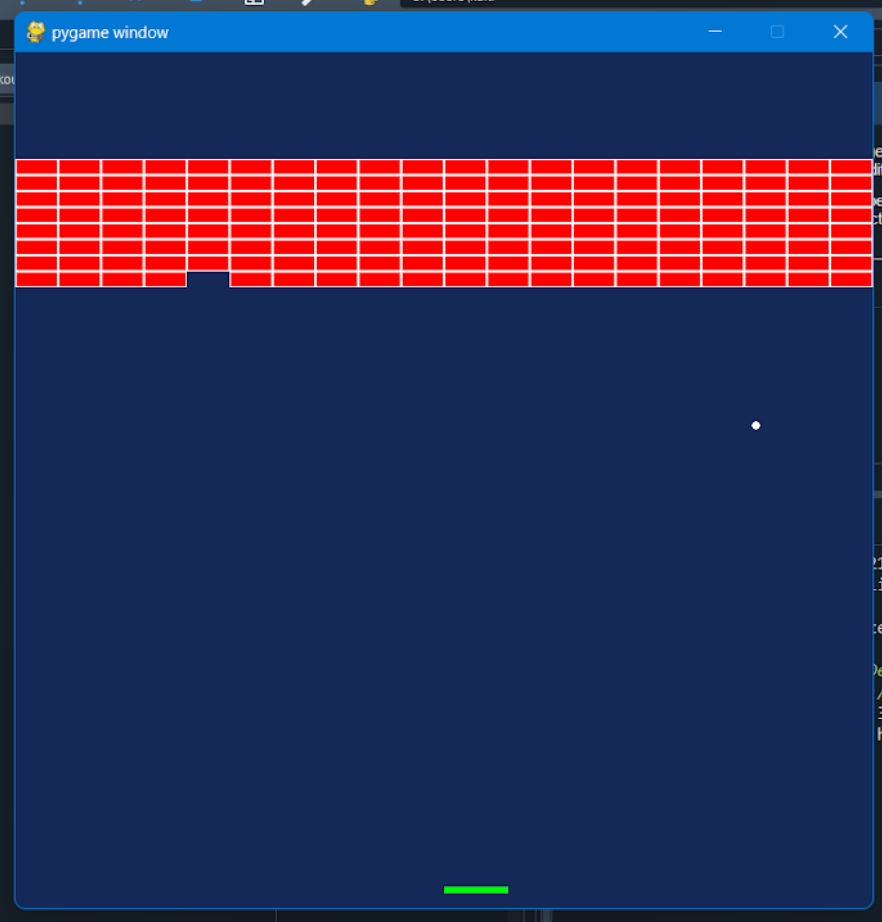
\includegraphics[width=4in]{images/Breakout_Screen.png}
\caption{Example breakout game running.}
\label{fig:Breakout_Screen}
\end{figure}

\begin{table}
\centering
\begin{tabular}{ |p{4cm}|p{1.5cm}|}
\hline
\multicolumn{2}{|c|}{Part List} \\
\hline
Part Description& Quantity \\
\hline
Adafruit Clue & 1 \\
AAA Battery Holder & 1 \\
USB Cable &1 \\
\hline
\multicolumn{2}{|c|}{Need 1 of the Items Below} \\
\hline
Buttons & 2 \\
Keyboard & 1 \\
\hline
\end{tabular}
\caption{The bill of materials for this project.}
\label{table:BOM}
\end{table}










\section{CONCLUSION}
Testing and practicing reflexes can be very important to those who have seen a decline in that action. To help test and improve reflexes our team decided a game would be a great test, not to mention fun so we have decided to base our game off of one of the classics, breakout. Even more convenient, our game will be portable so our users can improve their reflexes whenever they have a free moment. 

Our project will be programmed on the Adafruit Clue board and will utilize the screen and take user input through the buttons on the board. An important thing to ensure is that the game runs at the correct speed so that our main goal of improving and testing reflexes is effective. Overall our game will be an effective way of improving and testing reflexes, and will present challenges for our group in utilizing the screen, button inputs, and ensuring the game runs smoothly using the low power processor.

\section{REFERENCES}



\newpage
%\section{References}
\printbibliography
%\bibliographystyle{plain}
%\bibliography{ref}

\end{document}
